\documentclass[14pt,a4paper]{scrartcl}
\usepackage[utf8]{inputenc}
% \usepackage{fontspec}
% \setmainfont{Times New Roman}
\usepackage{showframe}
\usepackage{booktabs}
\usepackage{wrapfig}
\usepackage{hyperref}
% Example:
% \begin{wrapfigure}{R}{0.4\textwidth}
% \centering
% 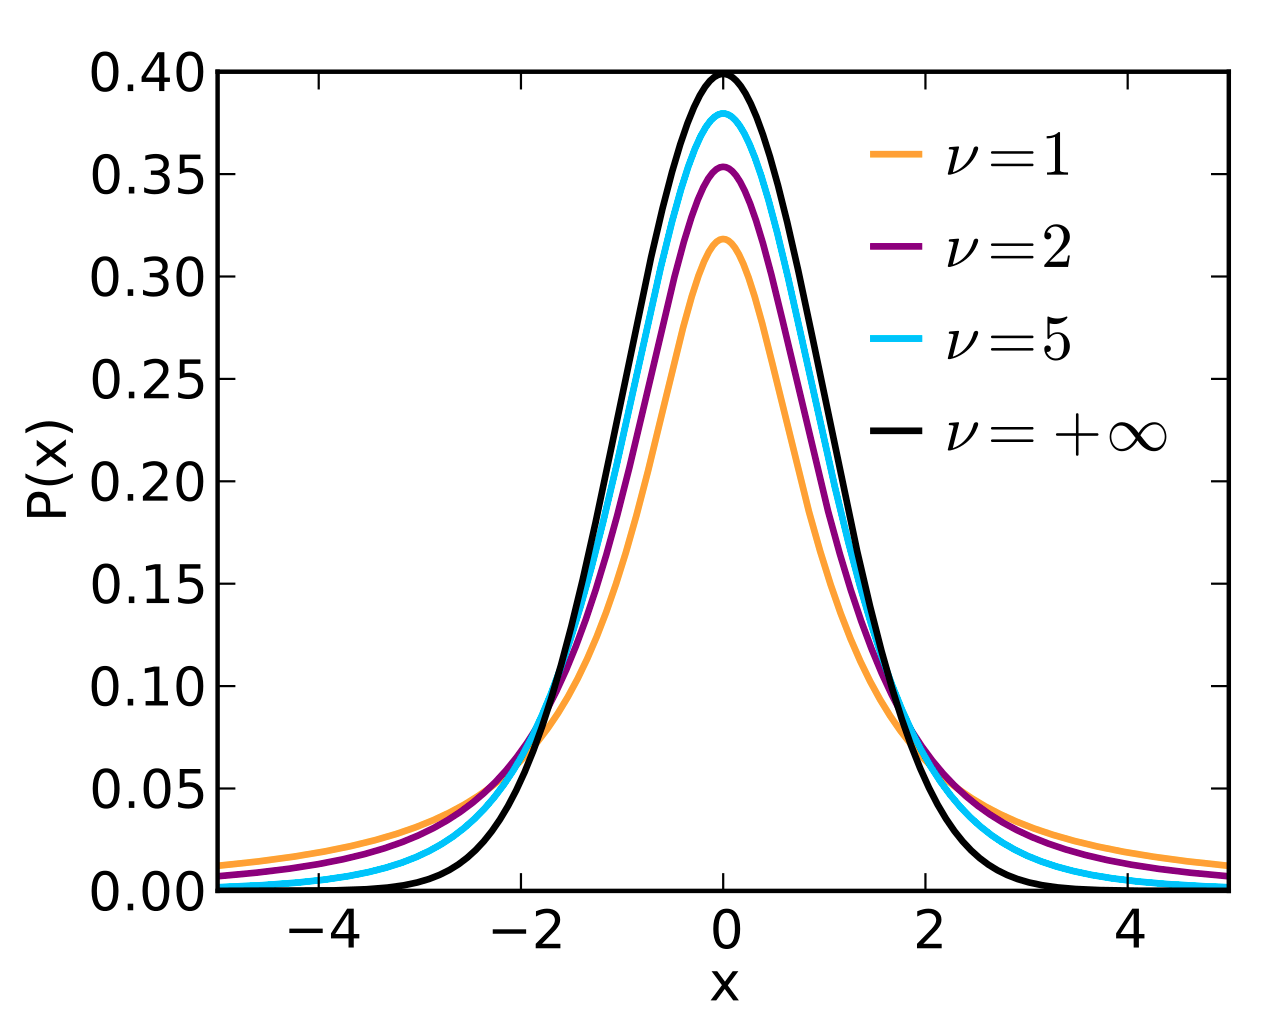
\includegraphics[width=0.35\textwidth]{assets/lectures_part_3-91d0349d.png}
% The PDF of the Student distribution.
% \end{wrapfigure}


\usepackage[english, russian, ukrainian]{babel}
\usepackage{misccorr,
            color,
            ragged2e,
            amsfonts,
            amsthm,
            graphicx,
            systeme,
            amsmath,
            mdframed,
            lipsum,
            mathtools,
            setspace
            }

\renewcommand\qedsymbol{$\blacksquare$}
\renewcommand*{\proofname}{\text{Доведення}}


\theoremstyle{definition}
\newtheorem*{defo}{Означення}
\newtheorem*{lemme}{Лема}
\newtheorem*{example}{Приклад}
\theoremstyle{remark}
\newtheorem*{remark}{Зауваження}
\theoremstyle{definition}
\newtheorem*{consequence}{Наслідок}
\theoremstyle{definition}
\newtheorem{statement}{Твердження}[section]
\newmdtheoremenv{boxteo}{Теорема}[section]

\setlength{\parindent}{0em}
\setlength{\parskip}{0.5em}
\DeclareMathOperator*\lowlim{\underline{lim}}
\DeclareMathOperator*\uplim{\overline{lim}}

\newcommand\independent{\protect\mathpalette{\protect\independenT}{\perp}}
\def\independenT#1#2{\mathrel{\rlap{$#1#2$}\mkern2mu{#1#2}}}

\usepackage{tikz}
\newcommand*\circled[1]{\tikz[baseline=(char.base)]{
  \node[shape=circle,draw,inner sep=1pt] (char) {#1};}}

% Default fixed font does not support bold face
\DeclareFixedFont{\ttb}{T1}{txtt}{bx}{n}{12} % for bold
\DeclareFixedFont{\ttm}{T1}{txtt}{m}{n}{12}  % for normal

% Custom colors
\definecolor{deepblue}{rgb}{0,0,0.5}
\definecolor{deepred}{rgb}{0.6,0,0}
\definecolor{deepgreen}{rgb}{0,0.5,0}

\usepackage{listings}

% Python style for highlighting
\newcommand\pythonstyle{\lstset{
language=Python,
basicstyle=\ttm,
morekeywords={self},              % Add keywords here
keywordstyle=\ttb\color{deepblue},
emph={MyClass,__init__},          % Custom highlighting
emphstyle=\ttb\color{deepred},    % Custom highlighting style
stringstyle=\color{deepgreen},
frame=tb,                         % Any extra options here
showstringspaces=false
}}


% Python environment
\lstnewenvironment{python}[1][]
{
\pythonstyle
\lstset{#1}
}
{}

% Python for external files
\newcommand\pythonexternal[2][]{{
\pythonstyle
\lstinputlisting[#1]{#2}}}

% Python for inline
\newcommand\pythoninline[1]{{\pythonstyle\lstinline!#1!}}

%                 USAGE:
% \begin{python}
% class MyClass(Yourclass):
%     def __init__(self, my, yours):
%         bla = '5 1 2 3 4'
%         print bla
% \end{python}
%
%
% \pythonexternal{demo.py}
%
%
% Definition \pythoninline{class MyClass} means \dots

\def\be{\begin{equation}}      % equation
\def\ee{\end{equation}}        % ...
\def\i{\infty}                 % infinity
\def\d{\partial}               % dx dy - partial     = \d
\def\bdash{\ \Big|\  }         % big vertical line   = |
\def\index{\mathbb{I}}         % indicator

\begin{document}


\begin{titlepage}
\centering
	\vspace{1cm}
	{ МІНІСТЕРСТВО ОСВІТИ І НАУКИ УКРАЇНИ\\
  НАВЧАЛЬНО-НАУКОВИЙ КОМПЛЕКС\\
  ``ІНСТИТУТ ПРИКЛАДНОГО СИСТЕМНОГО АНАЛІЗУ``\\
  НАЦІОНАЛЬНОГО ТЕХНІЧНОГО УНІВЕРСИТЕТУ УКРАЇНИ\\
  ``КИЇВСЬКИЙ ПОЛІТЕХНІЧНИЙ ІНСТИТУТ ІМЕНІ ІГОРЯ СІКОРСЬКОГО``\\
  КАФЕДРА МАТЕМАТИЧНИХ МЕТОДІВ  СИСТЕМНОГО АНАЛІЗУ\\\par}
	\vspace{5cm}
	{\large Розрахункова робота \\
	з курсу ``Математична статистика''
  \\
  \textbf{Варіант -- 126 (26)}
  \par}
	\vfill
  \begin{flushright}
  Виконав:\\
	студент КА-96\\
   Терещенко Денис, КА-96\\
  \end{flushright}


	\vfill

% Bottom of the page
	{\large КИЇВ - 2021 \par}
\end{titlepage}

\section*{Завдання варіанту.}
За вихiднi розподiли при отриманнi вибiрок
брались розподiли шести типiв:
\begin{itemize}
	\item гауссiвський,
	\item рiвномiрний,
 	\item експоненцiальний зi зсувом — щiльнiсть розподiлу має вигляд:
	\[
	 f_{\mathrm{Exp}} (\lambda, \alpha) = \begin{dcases}
	  \frac{1}{\lambda} e^{- \frac{x- \alpha}{\lambda}} , & x\geq \alpha;\\
		0 , & x < \alpha.
	 \end{dcases}
	\]
	\item бiномiальний,
	\item Пуассона,
	\item геометричний у формi \( p_{
	\mathrm{Geom} (\alpha)
	} (k)  = \frac{\alpha^k}{(\alpha+1)^{k+1}}, k \in \mathbb{N} \)
\end{itemize}
\begin{enumerate}
	\item Проведiть первинний аналiз вибiрки. Це включає статистичний ряд (для неперервних розподiлiв — iнтервальний), емпiричну функцiю розподiлу (для неперервних розподiлiв — iнтервальну), її графiк, полiгон частот (для дискретних розподiлiв), гiстограму (для неперервних розподiлiв), box-plot.
	\item Знайдiть вибiркове середнє, вибiркову дисперсiю, виправлену вибiркову дисперсiю, вибiркову медiану, вибiркову моду, вибiрковi коефiцiєнти асиметрiї та ексцесу.
	\item Обґрунтуйте та висуньте (нову) гiпотезу про розподiл генеральної сукупностi.
	\item Методом моментiв та методом максимальної вiрогiдностi знайдiть оцiнки параметрiв розподiлу.
	\item  Для кожного параметра кращу з цих двох оцiнок перевiрте на (асимптотичну) незмiщенiсть,
консистентнiсть та ефективнiсть.
	\item Побудуйте довiрчi iнтервали надiйнiстю 0.95 для параметрiв розподiлу.
\item Нарештi, перевiрте висунуту гiпотезу про розподiл генеральної сукупностi за допомогою
критерiю \( \chi^2 \) . Якщо гiпотеза суперечить вибiрковим даним, перейдiть до п. 3.
\item Висновок.
\end{enumerate}
\section{Первинний аналіз вибірки.}
Згідно з варіантом 126, маємо таку вибірку з $n = 100$ елементів:\par
4 3 5 4 5 4 0 2 4 4 5 2 4 4 4 4 3 5 4 5 3 5 4 4 3 5 4 2 5 4 6 5 2 2 3 2 2 4 3 3 3 2 4 3 5 3 4 4 6 3 4 4 4 5 5 3 3 3 3 6 4 3 2 2 4 5 1 5 3 5 4 1 2 4 4 3 3 5 2 3 5 5 4 5 4 5 3 2 5 3 6 6 4 4 3 2 4 4 4 1\par
Відсортована вибірка (варіаційний ряд) має вигляд (позначимо $ x_i, i = \overline{1, 100} $):\par
0 1 1 1 2 2 2 2 2 2 2 2 2 2 2 2 2 2 3 3 3 3 3 3 3 3 3 3 3 3 3 3 3 3 3 3 3 3 3 3 3 4 4 4 4 4 4 4 4 4 4 4 4 4 4 4 4 4 4 4 4 4 4 4 4 4 4 4 4 4 4 4 4 4 5 5 5 5 5 5 5 5 5 5 5 5 5 5 5 5 5 5 5 5 5 6 6 6 6 6\par
Бачимо, що розподіл г.с. є дискретним. Тодi нехай $x_1^* , \dots , x_m^*$ – елементи вибiрки, впорядкованi
за зростанням, причому кожне значення вказується лише один раз, $n_k$ – число разiв появи $x_k^*$ в реалiзацiї вибiрки.  $n_k$ називається \textit{частотою} появи $x_k^*$.\par
Зауважимо, що $n_1 + \dots + n_m = n$.\par
Сума частот елементiв $ \displaystyle\sum\limits_{i = 1}^{ \textit{k}}{x_i^*}$ називається \textit{кумулятивною частотою} $n_k^*$:
$$
n_k^* = n_1 + ... + n_k
$$
Величина $\nu_k = \dfrac{n_k}{n}$ називається \textit{вiдносною частотою}.\par
Сума вiдносних частот елементiв $\displaystyle  \sum\limits_{i = 1}^{k}{ \nu_i}$ називається \textit{кумулятивною
вiдносною частотою} елементу $x_k^*$. Отримаємо \textbf{статистичний ряд:}
\begin{center}
\begin{tabular}{|c|c|c|c|c|}
\hline
\begin{tabular}[c]{@{}c@{}}Значення \\ $(x_k^*)$\end{tabular} & \begin{tabular}[c]{@{}c@{}}Частоти \\ $(n_k)$\end{tabular} & \begin{tabular}[c]{@{}c@{}}Кумулятивнi \\частоти  $(n_k^*)$\end{tabular} & \begin{tabular}[c]{@{}c@{}}Вiдноснi частоти \\ $(\nu_k)$\end{tabular} & \begin{tabular}[c]{@{}c@{}}Кумулятивнi\\ вiдноснi\\ частоти $(\nu_k^*)$\end{tabular}  \\\hline
                 0 &                1 &                              1 &                        0.01 &                                      0.01 \\\hline
                 1 &                3 &                              4 &                        0.03 &                                      0.04 \\\hline
                  2 &               14 &                             18 &                        0.14 &                                      0.18 \\\hline
                  3 &               23 &                             41 &                        0.23 &                                      0.41 \\\hline
                  4 &               33 &                             74 &                        0.33 &                                      0.74 \\\hline
                   5 &               21 &                             95 &                        0.21 &                                      0.95 \\\hline
                   6 &                5 &                            100 &                        0.05 &                                      1.00 \\\hline
\end{tabular}
\end{center}
\newpage
\subsection*{Емпірична функція розподілу.}
\textit{Емпiричною функцією розподілу}, побудованою за вибiркою $\xi_1, \dots , \xi_n$ об’єму $n$, називається випадкова
функцiя $F_n^* : \mathbb{R} \times \Sigma \to [0,1]$ при кожному $y \in \mathbb{R}$ рiвна:
$$
F_n^* (y) = \frac{1}{n}  \sum\limits_{i = 1}^{ n}{ \index \left\lbrace \xi_i < y \right\rbrace}
$$
Побудуємо для нашої вибірки:
\[
F_{100}^* (y)= \begin{dcases}
0, &y \leq 0;\\
0.01, & 0 < y \leq 1;\\
0.04, & 1 < y \leq 2;\\
0.18, & 2 < y \leq 3;\\
0.41, & 3 < y \leq 4;\\
0.74, & 4 < y \leq 5;\\
0.95, & 5 < y \leq 6;\\
1, &  y > 6.\\
\end{dcases}
\]
\begin{center}
 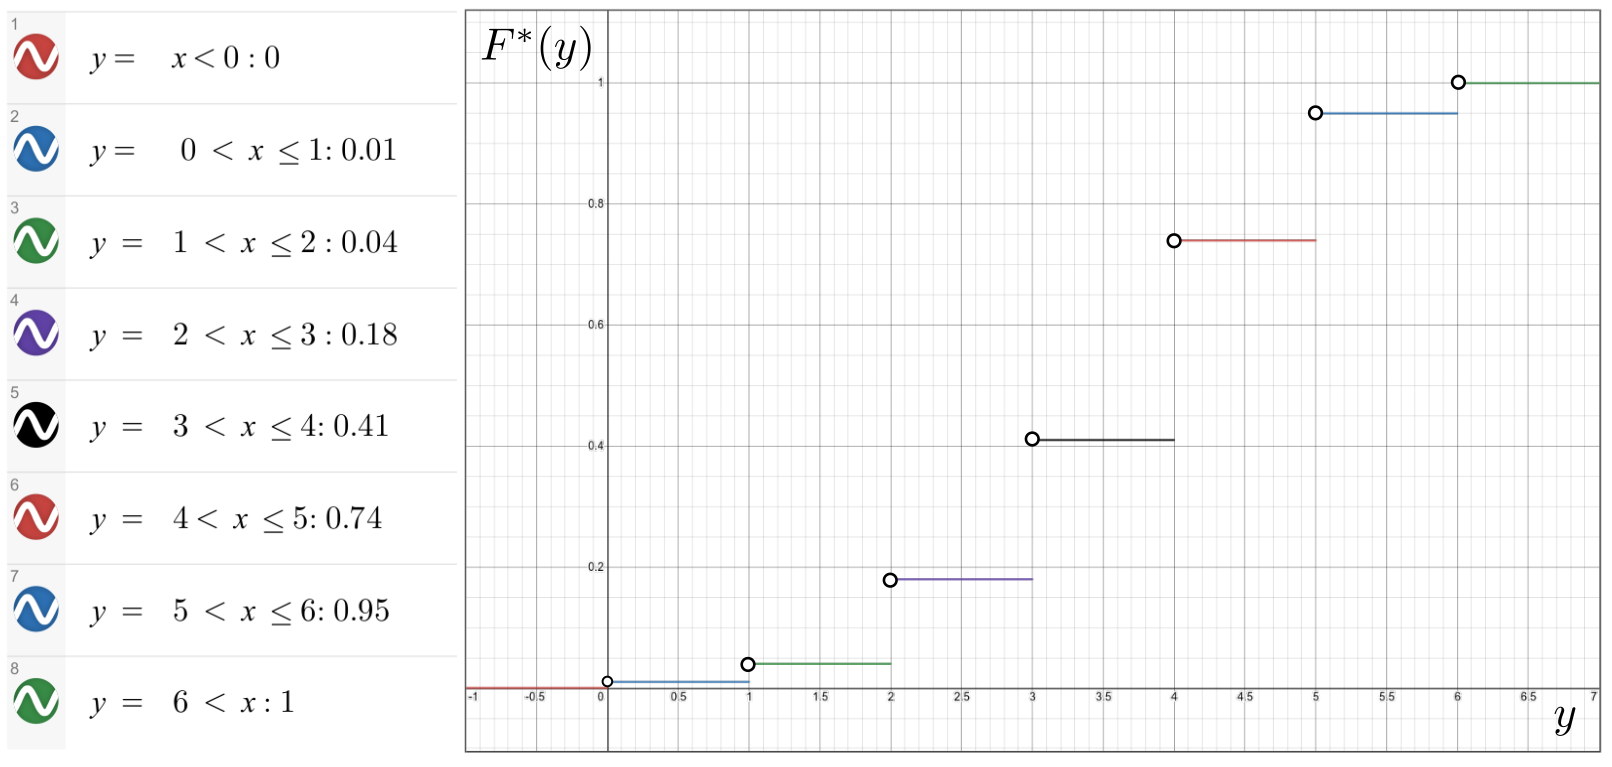
\includegraphics[scale=0.305]{assets/РР_126_Терещенко-7c0395e9.png}
\end{center}
\newpage
\subsection*{Полігон частот (count-plot).}
Якщо розподiл г.с. є дискретним, тодi полiгон частот будується на основi статистичного
розподiлу г.с. наступним чином: будують систему координат таку, що на осi абсцис будуть вiдображатися елементи вибiрки $x_1^*, \dots , x_m^*$, а на осi ординат вiдповiднi частоти.\par Далi у вказанiй системi координат будують точки $M_k (x_k^*, n_k), k= \overline{1,m}$, якi з’єднують
мiж собою у ламану $M_1M_2\dots M_m$.
\begin{center}
Полігон частот для заданої вибірки $x$
 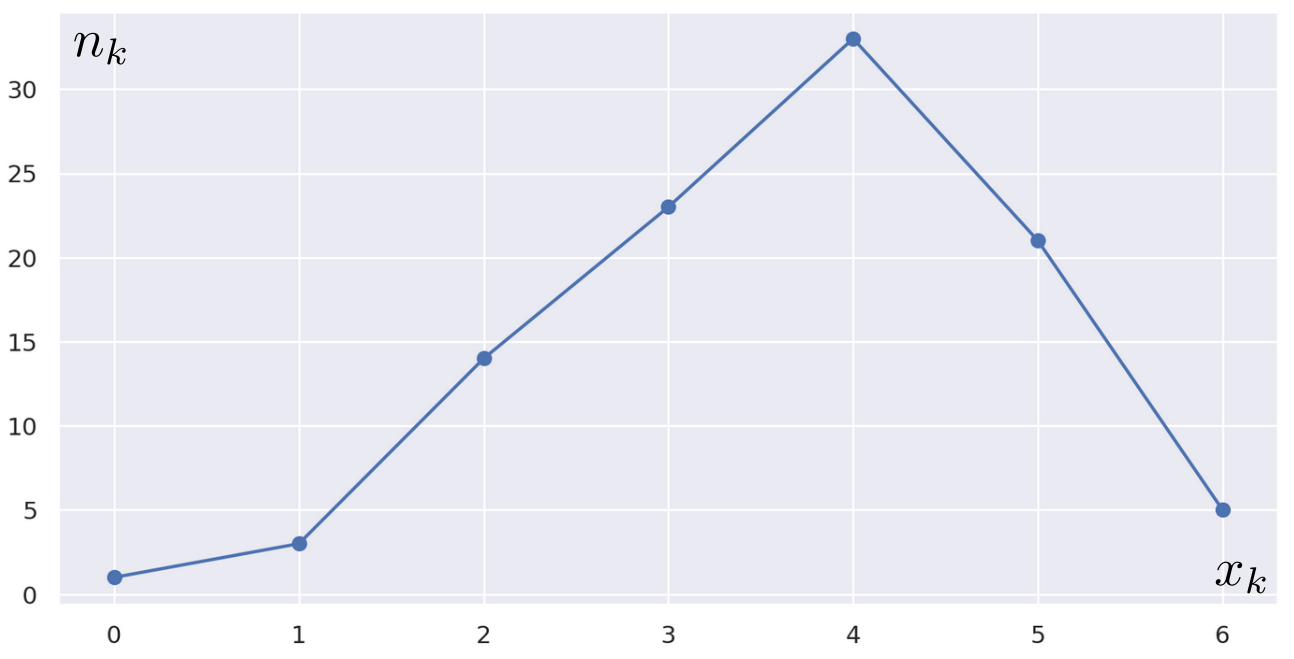
\includegraphics[scale=0.35]{assets/РР_126_Терещенко-d875be8e.png}
\end{center}
\subsection*{Boxplot.}
  \begin{center}
   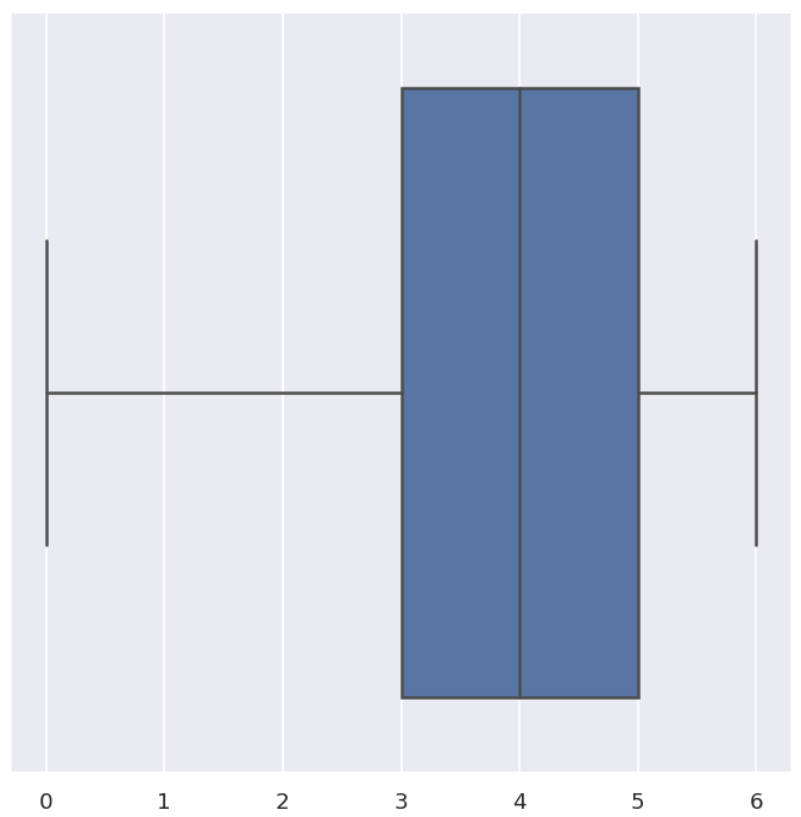
\includegraphics[scale=0.23]{assets/РР_126_Терещенко-cd2e904c.png}
  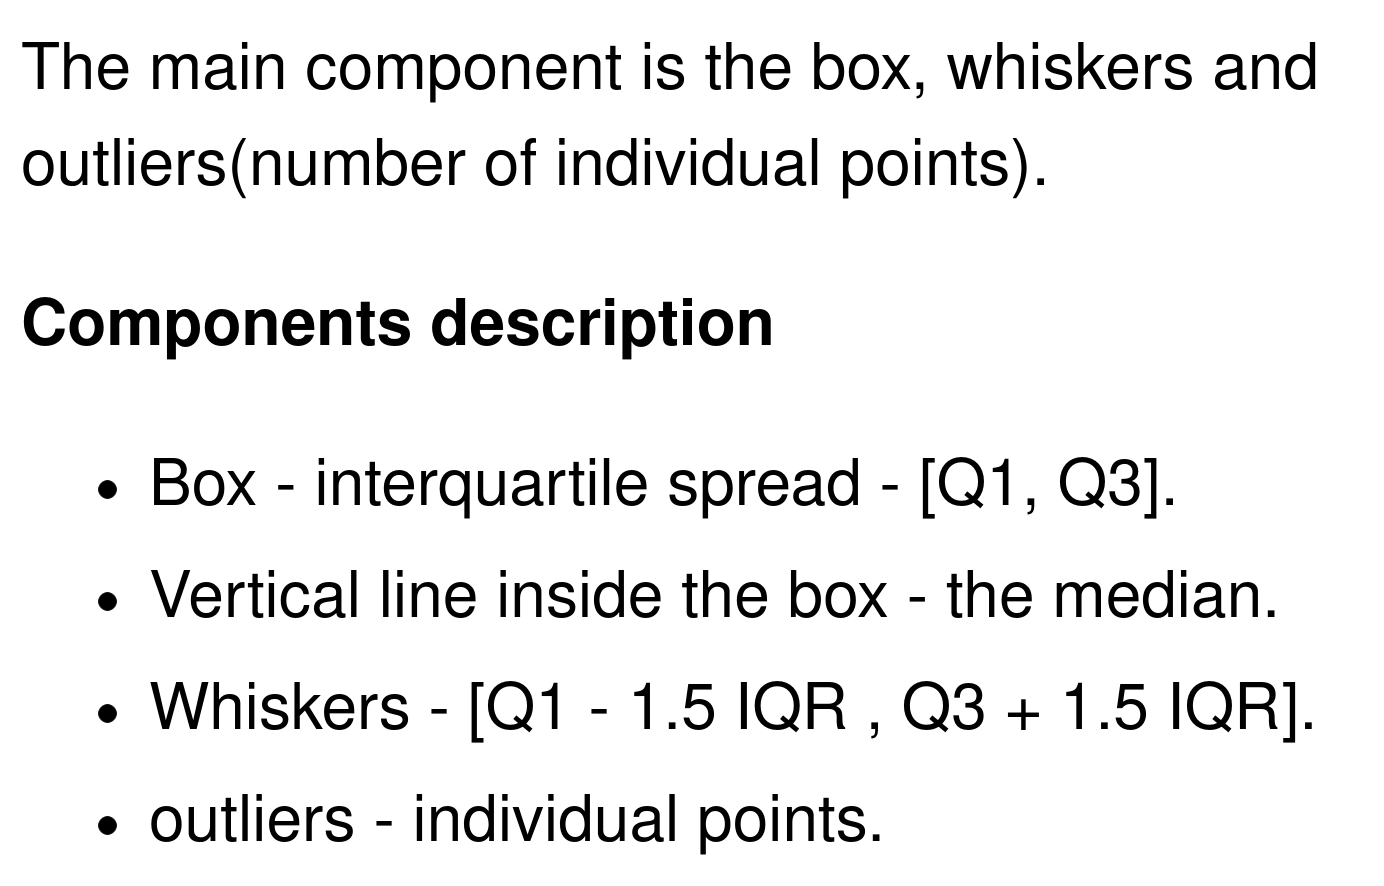
\includegraphics[scale=0.21]{assets/РР_126_Терещенко-539068e6.png}
  \end{center}
\newpage
\section{Дескриптивні міри.}
\textit{Знайдiть вибiркове середнє, вибiркову дисперсiю, виправлену вибiркову дисперсiю, вибiркову медiану, вибiркову моду, вибiрковi коефiцiєнти асиметрiї та ексцесу.}
\begin{itemize}
  \item Вибiркове середнє: \( \overline{x} = \frac{1}{100}  \sum\limits_{i = 1}^{100}{x_i} = \frac{367}{100} = 3.67 \)
  \item Вибіркова дисперсія: \( \mathbb{D}^{**}_\xi \approx \frac{152.11}{100} = 1.5211 \)
  \item Виправлена вибіркова дисперсія: \( \mathbb{D}^{***}_\xi = \frac{n}{n-1} \mathbb{D}^{**}_{\xi} \approx 1.5211 * \frac{100}{99} \approx 1.5364 \)
  \item Вибіркова мода -- очевидно, що найчастіше зустрічається \textbf{4} \( = M_o \)
  \item Вибіркова медіана: \( M_e = \dfrac{x_{50} + x_{51}}{2} = 4 \)
  \item Коефiцiєнт ассиметрії: \( A_s = \dfrac{\overline{\mu}_3}{\sigma^3} \approx \frac{-0.64817}{1.87601} \approx -0.3455 \)
  \item Коефіцієнт ексцесу: \( E_k = \dfrac{\overline{\mu}_4}{\sigma^4} - 3 \approx 2.8562 -3 = -0.14373 \)
  \end{itemize}
\textbf{Проміжний висновок:} розподіл скошено вліво (left skewed). Про це також свідчать положення вибіркових середнього та медіани. Усі значення у вибірці додатні, тож скористаємося коефіцієнтом варіації:
\[
 C_{V} =  \frac{\sqrt{\mathbb{D}_{\xi}^{***}}}{ \overline{x}} \cdot 100\% = 33\%
\]
Це свідчить про суттєве розсієння ознаки по відношенню до середнього показника. Також маємо від'ємний коефіцієнт ексцесу, тож розподіл більш ``пласковершинний'' ніж нормальний.
\newpage
\section{Гіпотеза.}
\textit{Обґрунтуйте та висуньте гiпотезу про розподiл генеральної сукупностi.} \par
Як було зауважено раніше, вибірка отримана з г.с. з дискретним розподілом. Розглянемо можливі варіанти:\par
  $ \  \bigcirc \ $ Poisson distribution. Має додатню ассиметрію (\( Sk = \lambda^{- \frac{1}{2}} \)) та додатній коефіцієнт ексцесу $ \lambda^{-1}, \lambda > 0$. Крім того, теоретичне значення середнього та дисперсії збігаються для розподілу Пуассона. Для нашої вибірки такі твердження будуть вкрай невірними. Таким чином, з великою ймовірністю вибірка прийшла не з розподілу Пуассона.\par
  $ \  \bigcirc \ $ Geometric distribution. Для геометричного розподілу за законом: \[ p_{
	\mathrm{Geom} (\alpha)
	} (k)  = \frac{\alpha^k}{(\alpha+1)^{k+1}}, k \in \mathbb{N} \] характерні додатні коефіцієнти ассиметрії та ексцесу: \( As = \frac{2 - p}{\sqrt{1-p}} \  Ek= 6 + \frac{p^2}{1 - p}  \). Також, теоретично мода геометричного розподілу дорівнює 1. Ці твердження не відповідають чисельним характеристикам нашої вибірки, тому навряд генеральна сукупність має геометричний розподіл. \par
  $ \  \bigcirc \ $ Найбільш логічним припущенням в данному випадку буде \textit{Біноміальний розподіл}. За чисельними характеристиками: від'ємний коефіцієнт ассиметрії та ексцесу свідчить, що $q < p$. Для порівняння теоретичного розподілу із розподілом вибірки, припустимо, за методом моментів, що:
  \[
   \xi \sim Bin(n, p) \quad \begin{gathered}
    \mathbb{E} \xi = \overline{x}\\
    \Downarrow\\
    np = \overline{x} = 3.67
   \end{gathered} \qquad \begin{gathered}
    \mathbb{D}_{\xi} = \mathbb{D}_{\xi}^{**}\\
    \Downarrow\\
     npq = 1.5211
   \end{gathered} \ \Longrightarrow \  \begin{cases}
    n = \lfloor \frac{a^2}{a-\sigma} \rfloor \approx  6 \\
    p = 1 - \frac{\sigma}{a } \approx   0.59
   \end{cases}
  \]
  За нашим припущенням г.с.: $\xi \sim Bin(6, 0.61)$. Чому саме 0.61 -- пояснимо далі.   Навідь за такої грубої оцінки отримали ``близькі'' параметри:
    \[
         As_{\xi} \approx - 0.31 \qquad Ek_{\xi} \approx - 0.29 \qquad Me_{\xi} = 4 \qquad Mo_{\xi} = \lceil 4.28 \rceil = 4
    \]
    \newpage
    Змоделюємо вибірку обсягом 100 із біноміального розподілу та порівняємо полігони частот заданої вибірки та отриманої:
    \begin{center}
    Згенеровані дані у порівнянні з заданою вибіркою:
     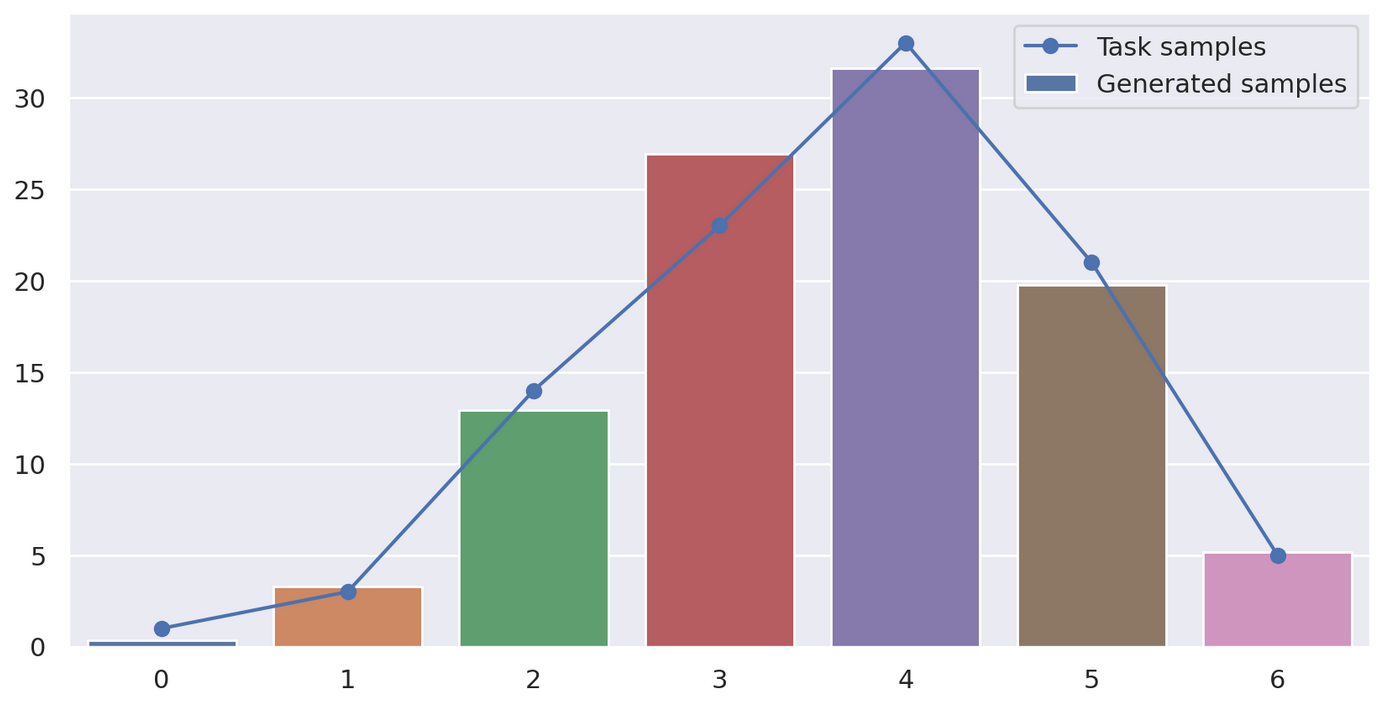
\includegraphics[scale=0.3]{assets/РР_126_Терещенко-8fcfc196.png}
    \end{center}
    \textbf{Проміжний висновок:} керуючись роздумами вище, можемо припустити, що г.с. має біноміальний розподіл. Пізніше більш корректно оцінемо параметри та перевіримо цю гіпотезу задопомогою критерію $\chi^2$. Остаточно сформулюємо:
    \begin{center}
     Гіпотеза \#1
     \[
     H_0 = \left\lbrace \xi \sim \mathrm{Bin}(n,p) \right\rbrace \qquad \quad
      H_1 = \left\lbrace \xi \nsim \mathrm{Bin}(n,p) \right\rbrace
     \]
    \end{center}
    де \( \xi \) -- вип. вел. Г.С., а параметри \( n,p \) -- оцінемо у подальшому.


  \newpage

\section{Оцінка параметрів.}
\subsubsection*{Метод моментів.}
Раніше виводили:
\[
 \xi \sim Bin(n, p) \quad \begin{gathered}
  \mathbb{E} \xi = \overline{x}\\
  \Downarrow \text{ м.м.}\\
  np = \overline{x} = 3.67
 \end{gathered} \qquad \begin{gathered}
  \mathbb{D}_{\xi} = \mathbb{D}_{\xi}^{**}\\
  \Downarrow \text{ м.м.}\\
   npq = 1.5211
 \end{gathered} \ \Longrightarrow \  \begin{cases}
  n = \lfloor \frac{a^2}{a-\sigma} \rfloor \approx 6 \\
  p = 1 - \frac{\sigma}{a } \approx 0.59
 \end{cases}
\]
Але, т.я. ми зменшуємо n, округлюючи вниз, то точніше буде рахувати \( p \) від n:
\[
 np = \overline{x} \quad \Longrightarrow \quad p = \frac{\overline{x}}{n} \approx 0.61
\]
\subsubsection*{MLE.}
Запишемо функцію вірогідності:
\[
\begin{split}
   \mathcal{L}(\overrightarrow{x}_m, n, p) &=  \prod\limits_{i=1}^{m}{f(x_i)} = \prod\limits_{i=1}^{m}{\left(\frac{n!}{{x}_{i}!\left(n-{x}_{i} \right)!} \right){p}^{{x}_{i}}{\left(1-p \right)}^{n-{x}_{i}} } =  \\
   &= \left( \prod_{i=1}^{m}\left(\frac{n!}{{x}_{i}!\left(n-{x}_{i} \right)!} \right)\right){p}^{\ \sum\limits_{i=1}^{m}{x}_{i}}{\left(1-p \right)}^{n-\sum\limits_{i=1}^{n}{x}_{i}}
\end{split}
\]
Опустимо перший множник, так як він не залежить від \( p \):
\[
  \ln \mathcal{L}(\overrightarrow{x}_m, n, p)=\sum_{i=1}^{n}{x}_{i} \ln(p)+\left(n-\sum_{i=1}^{n}{x}_{i} \right)\ln\left(1-p \right)
\]
\[
  \frac{\d\ln\mathcal{L}(\overrightarrow{x}_m, n, p)}{\d p}=\frac{1}{p}\sum_{i=1}^{n}{x}_{i}+\frac{1}{1-p}\left(n-\sum_{i=1}^{n}{x}_{i} \right)=0
\]
\[
 \left(1-p^*\right)\sum_{i=1}^{n}{x}_{i}+p^*\left(n-\sum_{i=1}^{n}{x}_{i} \right)=0 \ \Longrightarrow\    \fbox{\( \displaystyle
    p^*=\frac{\sum\limits_{i=1}^{n}{x}_{i}}{n}=\frac{\overline{x}}{n}
  \)}
\]
Маємо оцінку для $p$ при відомому $n$. Маючи достатньо велике $m=100$, виходячи з функції вірогідності, порівняно непоганою могла би бути оцінка:
\[
 n^* =  \max\limits_{i}{x^*_i} = 6
\]
Скористаємося літературою, яка описує оцінку параметрів при невідомих $n,p$:
\begin{center}
\href{https://www.stat.purdue.edu/~dasgupta/publications/binomialn.pdf}{Estimation of Binomial Parameters when Both n and p are Unknown}
\
 \\ A.DasGupta   Herman Rubin
 \\
 Purdue University \quad February 8,2004
\end{center}
Один з найпростіших підходів, які розглядаються (у наших позначеннях):
\[
  \max\limits_{i}{X^*_i} \xrightarrow[m\to\i]{a.s.} n
\]
Але, для застосування з прийнятною ймовірністю має бути: $m \geq 31500$. Слід зауважити, що у главі 2 (Nonexistence of Unbiased Estimates) представлено доведення відсутності незміщеної оцінки n при невідомих \( n,p \).\par
Скористаємося оцінкою $n$, яку пропонує автор матеріалу:
\[
  n^* = \frac{x^{\alpha +1}_{(k)} \cdot s^{2 \alpha}}{ \overline{x}^{\alpha} ( x_{(k)} -  \overline{x})^{\alpha}}
\]
де \(  x_{(k)} \) -- максимум вибірки, \( \alpha = \mathbb{P} \left\lbrace x_{(k)} < m \right\rbrace \). При підрахунку з $\alpha = 0.05$:
\[
 n^* \approx \lfloor  6.0039 \rfloor  = \mathbf{6}
\]
\textbf{Проміжний висновок:} таким чином, отримали вирази та чисельні оцінки для параметрів нашого гіпотетичного розподілу:
 \[
  n^* \approx 6 \qquad \quad p^* \approx 0,6116
 \]
 Як вже було зазначено, оцінка \( n \) є зміщеною, тобто не є ефективною. Тому, будемо перевіряти властивості оцінки \( p^* = \frac{\overline{x}}{n} \).
 \newpage
 \section{Властивості параметрів.}
 \subsubsection*{Незміщеність}
 \textit{Для кожного параметра кращу з цих двох оцiнок перевiрте на (асимптотичну) незмiщенiсть,
консистентнiсть та ефективнiсть.}
$\theta^*$ --- \textbf{незміщена} оцінка параметру $\theta$, якщо $\mathbb{E} \theta^* = \theta$.
\[
\mathbb{E} p^* = \mathbb{E} \left( \frac{\overline{x_m}}{n} \right) = \mathbb{E} \left( \frac{ \sum\limits_{i = 1}^{m}{\xi_i}}{mn} \right) =  \frac{nmp}{nm} = p \Longrightarrow \textit{ незміщена}
\]
\subsubsection*{Консистентність.}

\begin{defo} $\theta^*_n$ називається \textit{консистентною} оцінкою параметра $\theta$, якщо:
$$
\theta^*_n \xrightarrow[n\to\infty]{\mathbb{P}} \theta \quad \textit{--- слабка} \qquad \quad
\theta^*_n \xrightarrow[n\to\infty]{\text{м.н.}} \theta \quad \textit{--- сильна }
$$
\end{defo}

Для параметру \( p^*  \) за законом великих чисел маємо \textit{консистентність}:
\[
  \lim\limits_{m\to \i}  p^*_m =  \lim\limits_{m\to \i} \frac{ \frac{\xi_1 + \dots + \xi_m}{m}}{n} = \frac{1}{n}  \lim\limits_{m\to \i}  \frac{\xi_1 + \dots + \xi_m}{m} = \left| \text{м.н., ПЗВЧ} \right|  = \frac{1}{n} \mathbb{E} \xi = p
\]
\subsubsection*{Ефективність.}
Оцінка для \( n \) зміщена, тобто неефективна. \par
Якщо $\exists C_{m, p} : C_{m, p} \cdot(p^* - p) = \frac{\d \ln \mathcal{L} (\overline{x}, p)}{\d p}$, то оцінка  \( p^* \) буде ефективною:
\[
\begin{split}
  \frac{\d \ln \mathcal{L} (\overline{x}, p)}{\d p} & = \frac{ \sum\limits_{i=1}^{m}{x_i}}{p} - \frac{mn -  \sum\limits_{i=1}^{m}{x_i}}{1-p} = \frac{nmp^*}{p} - \frac{mn - mnp^*}{1-p} =  \\
  & = mn \left(  \frac{p^* - pp^* - p + pp^*}{p(1-p)} \right) = \frac{mn}{p(1-p)} (p^* - p)
\end{split}
\]
Отже,  \( p^*  = \dfrac{\overline{x}}{n}\) -- \textit{ефективна оцінка} параметра \( p \) т.я. $\exists C_{m, p} = \dfrac{mn}{p(1-p)} $.
\newpage
\section{Довірчі інтервали.}
Побудуємо довірчий інтервал надiйнiстю 0.95 для \( p^* = \frac{\overline{x}}{n} \), де n -- параметр біноміального розподілу, m -- кількість елеметів заданої вибірки \( \overrightarrow{x}_m = (x_1 \ \dots \ x_m) \).\par
При великих $m > 100$ за ЦГТ: \( p^* \approx N(\mathbb{E} p^*, \mathbb{D}p^*)  \Longrightarrow  \dfrac{p^* - \mathbb{E} p^*}{\sqrt{\mathbb{D}p^*}} \approx N(0,1)\).
\[
 \mathbb{E} p^* = p \ \text{(незміщеність)} \qquad \mathbb{D}p^* = \mathbb{D} \frac{\xi_1 + \dots \xi_m}{nm} = \frac{p - p^2}{m}
\]
\[
 \frac{(p^* - p)\sqrt{m}}{\sqrt{p - p^2}}  = \frac{p^* - p}{\sqrt{\frac{p - p^2}{m}}} \approx N(0,1)
\]
\[
\mathbb{P} \left\lbrace - t_{\gamma} <  \frac{(p^* - p)\sqrt{m}}{\sqrt{p - p^2}}  < t_{\gamma}  \right\rbrace \approx \gamma \qquad \Phi(t_\gamma) = \gamma/2 \Rightarrow t_{\gamma} = 1.96
\]
\[
  \frac{(p^* - p)^2 \cdot m }{p - p^2} < t_{\gamma}^2
  \quad \Longleftrightarrow  \quad
    mp^2 - 2mpp^* + m(p^*)^2 < t_{\gamma}^2\cdot(p - p^2)
\]
\[
    \left( 1 + \frac{ t_{\gamma}^2}{m} \right) p^2 - \left(2 p^* + \frac{ t_{\gamma}^2}{m} \right)p + (p^*)^2 < 0
\]
\def\tg{t_{\gamma}}
\def\pp{p^*}
\[
 D = 4 (p^*)^2 + 4 \frac{p^* t_{\gamma}^2}{m} +  \frac{ t_{\gamma}^4}{m^2} - 4 (p^*)^2 - 4  \frac{(p^*)^2 t_{\gamma}^2}{m} = t_{\gamma}^2 \left( \frac{4p^*}{m} + \frac{t_{\gamma}^2}{m} - \frac{4(p^*)^2}{m}  \right)
\]
\[
 p_{1,2} = \frac{2p^* + \frac{t_{\gamma}^2}{m} \pm \tg \sqrt{\frac{t_{\gamma}^2}{m} - \frac{4p^*(1 -\pp)}{m}} }{2 \left( 1 + \frac{\tg^2}{m} \right)}
\]
$m$ -- велике, тому можемо знехтувати \( \frac{\tg^2}{m}, \frac{\tg^2}{m^2}, \frac{2\tg^2}{m} \):
\[
 p_{1,2} \approx \frac{2p^* \pm \tg \sqrt{\frac{4p^*(1 -\pp)}{m}} }{2} = p^* \pm \tg \sqrt{\frac{p^*(1 -\pp)}{m}} = 0.6116 \pm 0.0956
\]
Отже, з довірчою ймовірністю \( \gamma = 0.95 \) параметр \( p \in (0.5160, 0.7071) \).
\newpage
\section{Перевірка гіпотези.}
\textit{Нарештi, перевiрте висунуту гiпотезу про розподiл генеральної сукупностi за допомогою
критерiю \( \chi^2 \) .} Виберемо рівень значущості $\alpha = 0.05$.
\[
 \begin{split}
  \text{Гіпотезa:} & \qquad \begin{gathered}
    H_0 = {\left\lbrace \text{Г.С. має біноміальний розподіл }  Bin(6, 0.6116) \right\rbrace}  \\
    H_1 = {\left\lbrace \text{Г.С. має НЕ біноміальний розподіл } Bin(6, 0.6116) \right\rbrace}
  \end{gathered}\\
  \text{Проміжки:} & \qquad \Delta_0 = \left\lbrace 0 \right\rbrace, \Delta_1 = \left\lbrace 1 \right\rbrace , \Delta_2 = \left\lbrace 2 \right\rbrace, \dots , \Delta_6 = \left\lbrace 6 \right\rbrace
 \end{split}
\]
Для біноміального розподілу розрахуємо ймовірності попадання у \( \Delta_k \) (PMF):
\[
 PMF: \quad \left( \begin{gathered}
  n\\
  k\\
 \end{gathered} \right) p^k q^{n-k} = P_k
\]
де \( p,n \) -- параметри розподілу, m -- кількість елементів вибірки, \( P_k \) -- ймовірність потрапляння у \( \Delta_k \).
\[
 \begin{array}{l|c|c}
 \  C(6,0)= 1.0 \
 & \  p^k \cdot q^{ n-k } \approx  0.00343 \   &
  \  P_k = 0.00343 \   \\ \hline
 \  C(6,1)= 6.0 \
 & \  p^k \cdot q^{ n-k } \approx  0.00541 \   &
  \  P_k = 0.03244 \   \\ \hline
 \  C(6,2)= 15.0 \
 & \  p^k \cdot q^{ n-k } \approx  0.00851 \   &
  \  P_k = 0.12769 \   \\ \hline
 \  C(6,3)= 20.0 \
 & \  p^k \cdot q^{ n-k } \approx  0.0134 \   &
  \  P_k = 0.26808 \   \\ \hline
 \  C(6,4)= 15.0 \
 & \  p^k \cdot q^{ n-k } \approx  0.02111 \   &
  \  P_k = 0.31661 \   \\ \hline
 \  C(6,5)= 6.0 \
 & \  p^k \cdot q^{ n-k } \approx  0.03324 \   &
  \  P_k = 0.19942 \   \\ \hline
 \  C(6,6)= 1.0 \
 & \  p^k \cdot q^{ n-k } \approx  0.05234 \   &
  \  P_k = 0.05234 \
 \end{array}
\]
\[
 \begin{array}{l|c|c|c|c|c|c|c}
   &\quad \Delta_0 \quad&\quad\Delta_1\quad&\quad\Delta_2\quad&\quad\Delta_3\quad&\quad\Delta_4\quad&\quad\Delta_5\quad&\quad\Delta_6\quad\\
   \hline
   n_k&1&3&14&23&33&21&5
   \\\hline
    m \cdot P_k & 0.343&  3.244& 12.769& 26.808& 31.661& 19.942&  5.234\\
 \end{array}
\]
Для більшості значень виконується \( mP_k >5 \). Обчислимо \( \chi^2 (m) \):
\[
 \chi^2 (100) \approx 1.2585 + 0.0184+ 0.1187+ 0.5409+ 0.0566+ 0.0561+ 0.0105 \approx 2.0596
\]
За теоремою Пірсона про критерій \( \chi^2 \):
\[
  \chi^2(100 ) \approx 2.0596 < 12.6 = \chi^2_{6, 0.05}
\]
Для порівняння, з іншим рівнем значущості \( \alpha = 0.95 \):
\[
  \chi^2(100 ) \approx 2.0596 < 2.17 = \chi^2_{6, 0.95}
\]
Таким чином, на вибраному рівні значущості \( \alpha = 0.05 \) гіпотеза \( H_0 \) не суперечить вибірковим даним.
\newpage
\section{Висновок.}
В ході виконання розрахункової роботи було проведено опрацювання, дослідження та аналіз заданої вибірки зі 100 елеметів. Результатом ранжування даних є наведений варіаційний ряд. Генеральна сукупність з великою ймовірністю є дискретною випадковою величиною. Проведено первинний аналіз вибірки шляхом побудови статистичного ряду, емпіриної функції розподілу:
\[
F_{100}^* (y)= \begin{dcases}
0, &y \leq 0;\\
0.01, & 0 < y \leq 1;\\
0.04, & 1 < y \leq 2;\\
0.18, & 2 < y \leq 3;\\
0.41, & 3 < y \leq 4;\\
0.74, & 4 < y \leq 5;\\
0.95, & 5 < y \leq 6;\\
1, &  y > 6.\\
\end{dcases}
\]
... та її графіка. За полігоном частот можна було передбачити від'ємний коефіцієнт ассиметрії та відносно великий розкид даних (що показує коефіцієнт варіації = 33\%). Це свiдчить про суттєве розсiєння ознаки по вiдношенню до середнього показника. Також маємо вiд’ємний коефiцiєнт ексцесу, тож розподiл бiльш “пласковершинний” нiж нормальний. Було розглянуто можливість 3х різних розподілів: пуассонівського, геометричного та біноміального. Перші 2 було відкинуто за несумісність з вибірковими даними (фактично, чисельні характеристики та форма графіків полігону частот та емпіричноїї функції розподілу є нехарактерними для даних розподілів). Для біноміального розподілу легко побачити схожість згенерованих даних з вибірковими.\par
Таким чином, була висунута гіпотеза про те, що вибірка прийшла з \textit{біноміального розподілу}.
Досить точною виявилася оцінка параметрів \( n, p \) методом моментів:
\[
 p^* = \frac{\overline{x}}{n} \qquad \quad     n = \lfloor \frac{a^2}{a-\sigma} \rfloor
\]
Оцінка \( p^* \) -- незміщена, консистентна, ефективна. Оцінка \( n \) -- зміщена. Далі побудували довірчі інтервали для \( p^* \): з довірчою ймовірністю \( \gamma = 0.95 \) параметр \( p \in (0.5160, 0.7071) \). \par  Внаслідок перевірки гіпотези \( H_0 = {\left\lbrace \text{Г.С.} =   Bin(6, 0.6116) \right\rbrace}  \) задопомогою
критерiю \( \chi^2 \), було встановлено, що на вибраному рівні значущості \( \alpha = 0.05 \) гіпотеза \( H_0 \) не суперечить вибірковим даним.
\end{document}
